\subsection{E4 (exploratory): LLM research agents}
We place open-weight instruction models, Qwen2.5-7B and Qwen2.5-72B \citep{qwen2024qwen25} served with vLLM, in the research loop over the 423 real strategies. Each turn the agent writes one sentence of reasoning and a JSON portfolio of up to 20 signals. It receives its training-period Sharpe (1970--1999) and either the validation Sharpe (status quo) or a sealed verdict. Each condition runs 8 episodes on actual data and 24 on null data. Every null episode uses its own bootstrap replicate, so its data are synthetic and pretraining knowledge of market history cannot help. We also give the 72B agent a \emph{batch tool} that evaluates up to 20 portfolios per turn for 15 turns, mimicking code-executing agents that run backtest sweeps. The status-quo report is the best-validation proposal, certified by ledger DSR over the \emph{distinct} proposals (duplicates are counted once, the convention used throughout).

\begin{table}[t]\centering\small
\caption{\textbf{E4.} LLM research agents (40 turns of one proposal, or 15 turns of up to 20 proposals with the batch tool; ``queries'' is the mean number of holdout queries actually made). Null rows: each episode uses its own bootstrap-null replicate, so every certification is false. Naive channel: report the best-validation proposal, certified by ledger DSR$>0.95$. Verdict channel: sealed PASS/FAIL with budget $K$ equal to the query allowance. Means over episodes.}\label{tab:e4}
\begin{tabular}{ll l cc ccc}\toprule
agent & data & channel & episodes & queries (distinct) & P(certify) & val.\ $t$ & test $t$\\\midrule
Qwen2.5-7B & actual & full Sharpe + DSR & 8 & 40 (22) & 0.000 & 1.99 & +0.33\\
Qwen2.5-7B & actual & sealed verdict & 8 & 39 (21) & 0.000 & -0.11 & -0.82\\
Qwen2.5-7B & null & full Sharpe + DSR & 24 & 39 (19) & 0.042 & 1.17 & +0.27\\
Qwen2.5-7B & null & sealed verdict & 24 & 38 (24) & 0.000 & -0.21 & +0.03\\
\midrule
Qwen2.5-72B & actual & full Sharpe + DSR & 8 & 40 (29) & 0.000 & 1.58 & +0.15\\
Qwen2.5-72B & actual & sealed verdict & 8 & 40 (29) & 0.000 & 0.72 & +0.08\\
Qwen2.5-72B & null & full Sharpe + DSR & 24 & 40 (30) & 0.042 & 1.21 & +0.09\\
Qwen2.5-72B & null & sealed verdict & 24 & 31 (26) & 0.000 & 0.02 & +0.01\\
\midrule
72B + batch tool & actual & full Sharpe + DSR & 8 & 63 (36) & 0.125 & 2.32 & -0.39\\
72B + batch tool & actual & sealed verdict & 8 & 53 (44) & 0.000 & 0.37 & +0.27\\
72B + batch tool & null & full Sharpe + DSR & 24 & 93 (35) & 0.000 & 1.77 & +0.16\\
72B + batch tool & null & sealed verdict & 24 & 76 (62) & 0.000 & 0.15 & +0.19\\
\bottomrule\end{tabular}\end{table}


Table~\ref{tab:e4} and Figure~\ref{fig:agents} give a more nuanced picture than Theorem~\ref{thm:attack} alone. Qualitatively, the 72B agent does exactly what the theory describes. With the batch tool it writes, for example, \emph{``The combination of hold\_Aero and tsmom\_Aero\_63 shows the highest validation Sharpe. Testing further variations and adding other promising signals''}, and it grows an ensemble of validation winners turn by turn, which is greedy forward selection on the holdout. Quantitatively, today's agents are \emph{inefficient} adaptive analysts. The single-proposal agents converge within about 15 turns: the 7B model makes 19--22 distinct proposals in 40 turns and the 72B model 29--30, after which they resubmit near-identical portfolios. The batch agent uses its full 15 turns but submits only about 6 portfolios per turn rather than the 20 allowed, a median of about 70 queries (35 distinct) on the null. Their best null validation $t$ plateaus at 1.2--1.8, whereas the scripted greedy analyst of E1 reaches $t\approx4$--$6$ with a comparable number of queries (40--100). Ledger DSR therefore certified only 2 of 72 null status-quo episodes (2.8\%, both from single-proposal agents), within the nominal 5\%. Neither certification is driven by adaptivity. Both have validation $t$ ($2.64$ and $2.99$) at the Bonferroni bar for their number of distinct proposals, and are certified because highly correlated proposals shrink DSR's scale estimate ($nV=0.37$ and $0.11$). This is a second, non-adaptive weakness of ledger DSR (Corollary~\ref{cor:instances}(i)). On actual data one batch episode is certified (validation $t=3.30$, DSR $0.99$, $nV=0.21$) and then has test $t=-0.63$ over 2013--2026.

The honest reading is that \emph{chat-style} LLM agents do not yet exploit a holdout within a single session. The adaptive capacity is there for any agent that searches more efficiently, for example by writing code, running for longer, or being trained to search. The sealed verdict made no false certifications in any condition and costs nothing in these settings.

\begin{figure}[t]
\centering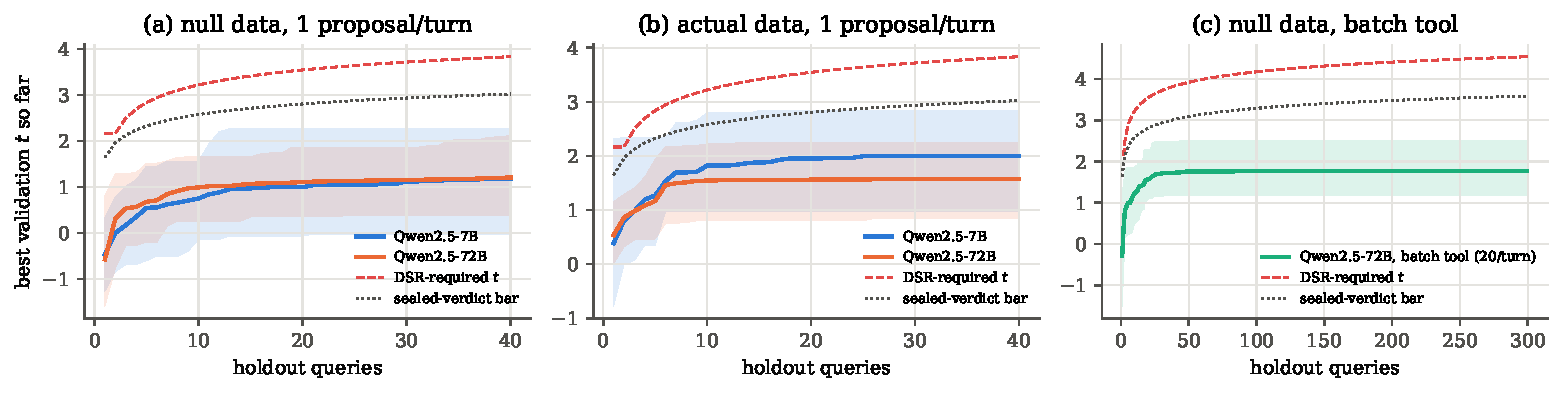
\includegraphics[width=\linewidth]{../figures/fig4_agents.pdf}
\caption{\textbf{E4.} Best validation $t$ found so far by LLM agents under the full-Sharpe channel (mean and 10--90\% band over episodes), against the $t$ that ledger DSR requires and the sealed-verdict bar for the same number of queries.}
\label{fig:agents}
\end{figure}

\subsection{E5 (exploratory): RL alpha mining with GRPO}
RL alpha miners optimise a backtest metric directly \citep{yu2023alphagen}, which makes them the most aggressive adaptive analysts in practice. We fine-tune Qwen2.5-1.5B-Instruct with GRPO \citep{shao2024deepseekmath} (LoRA rank 32, learning rate $5\times10^{-5}$, 300 steps $\times$ 32 completions $=9{,}600$ scored portfolios). The policy emits one JSON portfolio per completion, and invalid outputs receive $-1$. We compare three rewards: the portfolio's validation Sharpe (\emph{val}); its training Sharpe with the holdout sealed (\emph{train}); and an AlphaGen-style \emph{pool} reward, the marginal improvement in validation Sharpe of a growing combined portfolio, into which the batch's best improver is merged each step \citep{yu2023alphagen}. The pool reward is the RL analogue of Theorem~\ref{thm:attack}.

\begin{table}[t]\centering\small
\caption{\textbf{E5.} GRPO on Qwen2.5-1.5B, 300 steps $\times$ 32 completions; s2 and s3 are additional seeds (fresh null replicate and RL seed). Reported strategy: the best distinct portfolio by the reward split. Validation-reward runs are certified by ledger DSR over all distinct portfolios; the pool run reports the final pool, with the ledger comprising all distinct portfolios and pool states; train-reward runs by the sealed verdict over the 40 best-by-train portfolios.}\label{tab:e5}
\begin{tabular}{ll ccc cc}\toprule
data & reward & distinct portfolios & val.\ $t$ & test $t$ & DSR & certified\\\midrule
null & validation & 200 & 3.87 & +0.40 & 0.680 & no\\
null & validation (s2) & 2450 & 2.48 & +0.28 & 0.522 & no\\
null & validation (s3) & 364 & 2.34 & -0.61 & 0.339 & no\\
null & train (sealed) & 106 & -0.57 & -0.22 & -- & no\\
null & validation pool & 300 & 4.12 & +0.74 & 0.763 & no\\
null & validation pool (s2) & 202 & 2.86 & -0.38 & 0.695 & no\\
null & validation pool (s3) & 9201 & 12.01 & -0.56 & 1.000 & yes\\
actual & validation & 1409 & 5.00 & -0.26 & 0.948 & no\\
actual & train (sealed) & 3151 & 0.10 & +0.13 & -- & no\\
\bottomrule\end{tabular}\end{table}


Table~\ref{tab:e5} and Figure~\ref{fig:grpo} show that, in every run (one seed per arm), the RL miner overfits the split it is rewarded on. With validation reward on the null, the policy finds a portfolio with validation $t=3.87$ within about 10 steps and collapses onto it (test $t=+0.40$). On actual data the mean validation Sharpe of its samples rises for about 120 steps. The best portfolio, first generated at step 187, has validation $t=5.00$ (a 2000--2012 annualised Sharpe of 1.39) and then \emph{loses money} over 2013--2026 (test $t=-0.26$). Ledger DSR over the 1,409 distinct portfolios it evaluated gives $0.948$: DSR declines to certify, but by a margin of $0.002$. The pool reward produces a combined portfolio with validation $t=4.12$ within 21 steps (DSR $0.763$ over all distinct portfolios and pool states). The pool, however, is not the many-signal noise ensemble of Theorem~\ref{thm:attack}. Six of its seven signals are variants of a single industry (Aero), so the policy has found one spurious industry and re-weighted it. It then loses entropy and stops proposing improvers, and the pool does not change after step 21.

With training reward and the holdout sealed, the RL miner overfits the \emph{training} period instead. On actual data it converges to a basket of 5- and 21-day industry momentum signals with a 1970--1999 annualised Sharpe of 4.3, consistent with the strong short-horizon autocorrelation of pre-2000 daily industry returns. Its validation and test Sharpe are about zero. The sealed verdict over the 40 best-by-training portfolios correctly certifies nothing in either train-reward run.

As with LLM agents, the RL policies substantially inflate validation performance relative to test performance, but GRPO's mode collapse caps how many distinct holdout queries they effectively make (106--3,151 distinct portfolios out of 9,600 completions). In this configuration ledger DSR is not defeated, although in one run its margin is $0.002$. The sealed reward makes validity independent of such optimiser details.


\begin{figure}[t]
\centering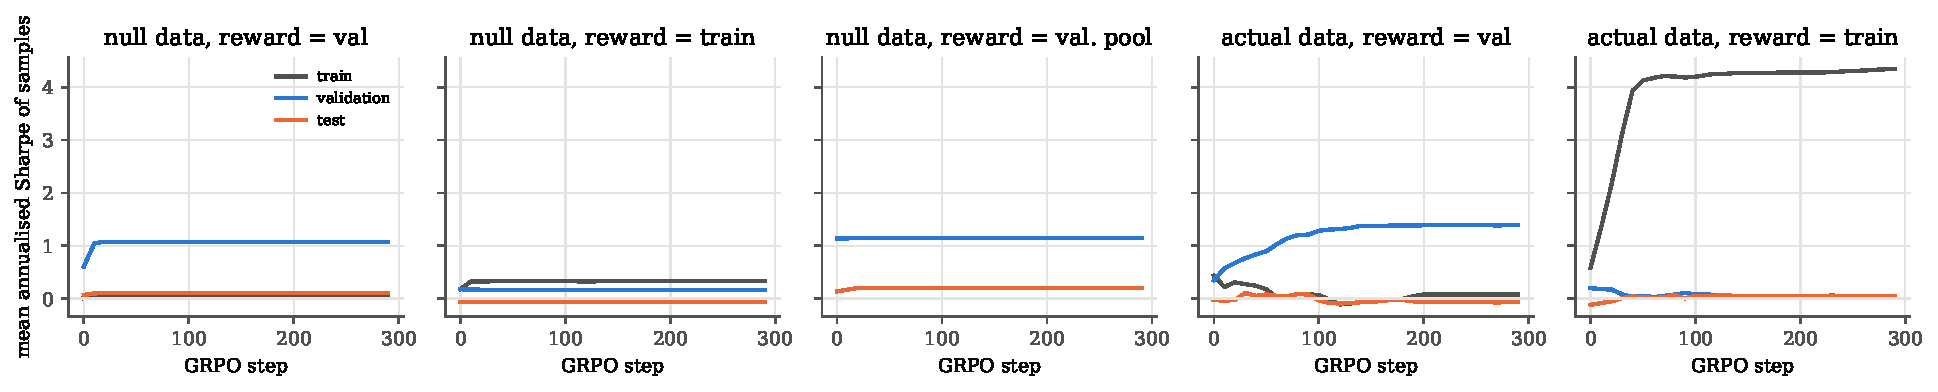
\includegraphics[width=\linewidth]{../figures/fig5_grpo.pdf}
\caption{\textbf{E5.} Mean annualised Sharpe of sampled portfolios on the training, validation and test splits during GRPO training (10-step bins).}
\label{fig:grpo}
\end{figure}
